\documentclass[10pt,conference]{IEEEtran}
\IEEEoverridecommandlockouts
\usepackage[spanish,es-tabla]{babel}
\renewcommand{\baselinestretch}{1.5}     %interlineado
\usepackage[utf8]{inputenc} 
\usepackage[square,numbers]{natbib}
\bibliographystyle{abbrvnat}
\usepackage{float}                      % para usar [H]
\usepackage[table,xcdraw]{xcolor}
\usepackage{amsmath,amssymb,amsfonts}
\usepackage{graphicx}
\usepackage{textcomp}
\usepackage{xcolor}
\usepackage{ragged2e} % \justify

%---------- pie de pagina
\usepackage{fancyhdr}
\pagestyle{fancy}
\fancyhf{}
\rfoot[]{\thepage}
%-----------------
\def\BibTeX{{\rm B\kern-.05em{\sc i\kern-.025em b}\kern-.08em
    T\kern-.1667em\lower.7ex\hbox{E}\kern-.125emX}}
%__________

\title{Estrategias de búsqueda \\ {\Large Inteligencia Artificial}}
%--------------------------------------------
\author{
\IEEEauthorblockN{1\textsuperscript{do} Angely Mendez}
\IEEEauthorblockA{\textit{Escuela de Informática} \\
\textit{Universidad Nacional de Trujillo}\\
Trujillo, Perú \\
t052701020@unitru.edu.pe}
\and
\IEEEauthorblockN{2\textsuperscript{ero} Ciara Mendez}
\IEEEauthorblockA{\textit{Escuela de Informática} \\
\textit{Universidad Nacional de Trujillo}\\
Trujillo, Perú \\
t022700920@unitru.edu.pe}
}

%%--------------------------------------------
\begin{document}
\renewcommand{\IEEEkeywordsname}{{\bfseries Palabras claves:}} % Colocar Keywords en Spanish

\maketitle
%-------------------------------------------
\begin{abstract}
Este documento es una investigación que describe cinco de las estrategias de búsqueda en el área de Inteligencia Artifical, las cuales se dividen en búsquedas no informadas y son: Búsqueda en amplitud(BFS), Búsqueda en profundidad(DFS), Búsqueda de costo uniforme(UCS) e informadas: Búsqueda voraz (greedy) y Búsqueda A*. Las cuales realizan acciones mecanizadas o resuelven problemas, reduciendo a buscar en un espacio de estados. Por lo que en este artículo se define y explica a que se refiere cada búsqueda, además se menciona una investigación que aplica dicha estrategia y cómo es útil usarlos en implementaciones para beneficio de la sociedad.   
\end{abstract}

\begin{IEEEkeywords}
Estrategias de búsqueda, inteligencia artificial.
\end{IEEEkeywords}

\section{\textbf{Introducción}}
El tema de búsquedas en inteligencia artificial(IA) es prioritario, dado que al realizar acciones mecanizadas o resolver problemas, se reduce a buscar en un espacio de estados. Estas búsquedas utilizan dominios como la deducción, elaboración de planes de actuación, razonamientos de sentido común, prueba automática de teoremas, etc.

En la disciplina de la IA se estudian búsquedas no informadas o ciegas (búsqueda primero en amplitud, primero en profundidad, profundidad iterativa, de costo uniforme, etc.) y búsquedas informadas o inteligentes (búsqueda avara, A*, IDA*, A* restricta por memoria simplificada, ascenso de cima (hill-climbing), etc.)

En este informe se presenta información al respecto, el cual está organizado de la siguiente manera: en primer lugar, se explican los conceptos teóricos: definiciones de cada una de las estrategias, luego se da énfasis en una investigación que está relacionada con ellas y para finalizar las conclusiones más relevantes.
%------------------------------------------
\section{\textbf{Estrategias de búsqueda}} 
%\vspace{-22 mm}

\subsection{\underline{\textbf{Búsqueda primero en amplitud (BFS)}}}
Es un algoritmo para atravesar o buscar estructuras de datos de árboles o gráficos. Explora todos los nodos en la profundidad actual antes de pasar a los nodos en el siguiente nivel de profundidad. \citep{amplitud}
Un algoritmo de búsqueda primero en amplitud busca horizontalmente. La siguiente Figura ~\ref{f1} demuestra esto:

\begin{figure}[H]
 \begin{center}
       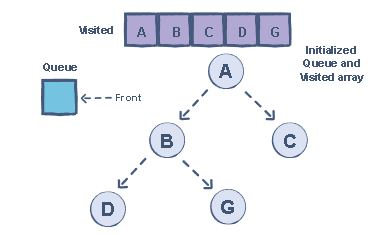
\includegraphics[width=5cm, height=3cm]{figuras/1.JPG}
      \caption{Ejemplo de Grafo dirigido para Búsqueda en Amplitud .}
      \label{f1} 
      \end{center}
\end{figure}

En la Figura ~\ref{f1} tenemos un gráfico dirigido de cinco nodos, siendo G el nodo a buscar. Los nodos se marcarán como visitados utilizando la \textit{visited} matriz, mientras que los nodos adyacentes se agregarán a la \textit{queue}.

\citep{ventajasamplitud} menciona las siguientes ventajas:
\begin{itemize}
    \item Si sabemos que una respuesta estará cerca del nodo raíz, un BFS es más eficiente. Por ejemplo, en el ejemplo del árbol genealógico, podríamos estar buscando un descendiente directo que vivió 50 años después que el antepasado en el nodo raíz, no 300 años después.
    \item Los BFS son excelentes para calcular la ruta más eficiente entre dos nodos. Por esa razón, son excelentes para aplicaciones de GPS y mapas e incluso para encontrar personas cercanas en las redes sociales.
\end{itemize}

A continuación, una investigación respecto a la Búsqueda en Amplitud:
\begin{enumerate}
\item En su Tesis \textit{“Diseño, implementación y aplicación de una estrategia de búsqueda preferente por amplitud, para uso multidireccional sobre sistemas distribuidos o de procesamiento en paralelo, usando un simulador de escenarios, construido para el trazado de rutas en robótica móvil.”} Maestría en Instrumentación Física. Universidad Tecnológica de Pereira. Pereira-Colombia; \citep{gonzalez} plantea la construcción de un simulador de escenarios en dos dimensiones, el cual permitirá que un robot de software (llamado Softbot) y los diferentes elementos que conforman un ambiente, se utilicen como sistema de pruebas en la búsqueda de una ruta apropiada para ir de un punto a otro. Como herramienta para la determinación de la ruta se utilizan técnicas de Inteligencia Artificial (IA), lo que se logra mediante la sucesión de cambios de estado a través de acciones o transformaciones, el uso de estrategias de búsqueda (Ver Figura ~\ref{f4}) y heurísticas generales.Finalmente se implementa la capacidad de interactuar no solo uno, sino varios agentes de software, trabajando en forma cooperativa, de tal forma que con la ayuda de ellos y aplicando la estrategia de búsqueda multidireccional sea posible establecer una ruta.
\begin{figure}[H]
 \begin{center}
       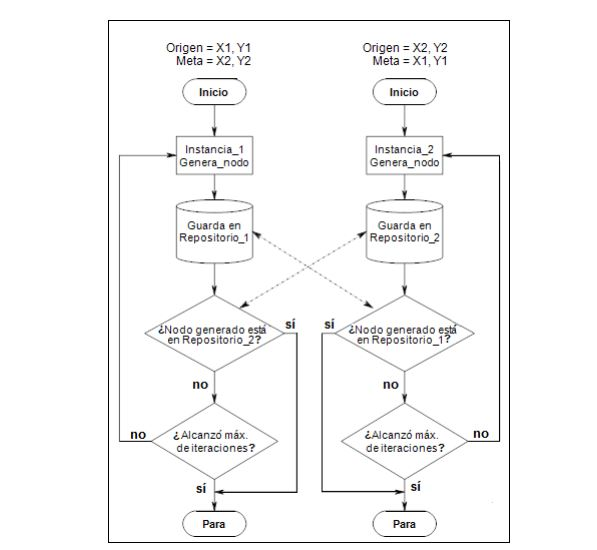
\includegraphics[width=8cm, height=5cm]{figuras/4.JPG}
      \caption{Algoritmo de la búsqueda preferente por amplitud bidireccional.}
      \label{f4} 
      \end{center}
\end{figure}
\end{enumerate}
%---------------------------------------------------------------------------
\subsection{\underline{\textbf{Búsqueda en profundidad (DFS)}}}
Es un algoritmo para atravesar o buscar estructuras de datos de árboles o gráficos que utiliza la idea de retroceder. Explora todos los nodos avanzando si es posible o retrocediendo.\citep{profundidad}
La siguiente Figura ~\ref{f2} demuestra esto:

\begin{figure}[H]
 \begin{center}
       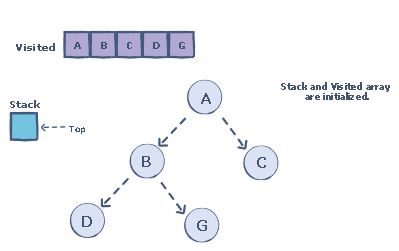
\includegraphics[width=6cm, height=4cm]{figuras/2.JPG}
      \caption{Ejemplo de Grafo dirigido para Búsqueda en Profundidad .}
      \label{f2} 
      \end{center}
\end{figure}

En la Figura ~\ref{f2} Tenemos un gráfico dirigido de cinco nodos, siendo G el nodo a buscar. Los nodos se marcarán como visitados utilizando la \textit{visited} matriz, mientras que los nodos adyacentes se agregarán a \textit{lastack}.


\citep{ventajasamplitud} menciona las siguientes ventajas:
\begin{itemize}
    \item Los DFS son excelentes para crear juegos porque permiten que el algoritmo explore las posibilidades de ganar y perder.
    \item Si sabemos que la respuesta que buscamos estará en la parte inferior de un árbol, un DFS normalmente será más rápido que un BFS. Por ejemplo, podríamos estar buscando descendientes vivos de un árbol genealógico largo, y todos los vivos estarán en la parte inferior del árbol.
    \item DFS suele ocupar menos memoria que BFS.
\end{itemize}

A continuación, una investigación respecto a la Búsqueda en Profundidad:
\begin{enumerate}
\item En la Tesis \textit{“Modulo de creación de laberintos en Unity”} Ingeniería Informática. Universidad Autónoma de Madrid. Madrid-España; \citep{montero} se basa en poder proporcionar la misma facilidad para un usuario de crear laberintos aleatorios como la que se proporciona por el entorno de desarrollo mediante interfaz. Para ello se han creado unos scripts en donde se encapsulan las necesidades más imprescindibles que puede tener un usuario a la hora de crear un laberinto. Los algoritmos de generación de laberintos son varios, pensados para distintas necesidades de generación, cada cual tiene sus pros y sus contras. En este caso el Algoritmo DFS ( Ver Figura ~\ref{f3}), también conocido como búsqueda primero en profundidad, el cual genera un laberinto tradicional perfecto en donde no existen zonas cerradas a las cuales no se pueda acceder y no posee bucles por lo que si se recorriese siempre el lado izquierdo o derecho del laberinto se alcanzarían todas las zonas sin importar la forma del laberinto.
\begin{figure}[H]
 \begin{center}
       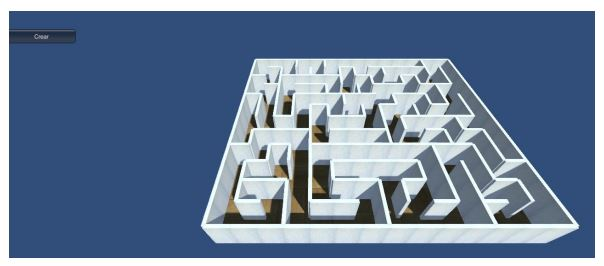
\includegraphics[width=5cm, height=3cm]{figuras/3.JPG}
      \caption{Laberinto con generación de algoritmo búsqueda en profundidad.}
      \label{f3} 
      \end{center}
\end{figure}
\end{enumerate}
%---------------------------------------------------------------------------
\subsection{\underline{\textbf{Búsqueda de costo uniforme (UCS)}}}
Es un algoritmo de búsqueda no informado que utiliza el costo acumulativo más bajo para encontrar una ruta desde el origen hasta el destino. Los nodos se expanden, comenzando desde la raíz, de acuerdo con el costo mínimo acumulativo \citep{coste}. 

A continuación se muestra un ejemplo de UCS en acción. Usaremos el gráfico (Ver Figura ~\ref{fcoste1}):

\begin{figure}[H]
 \begin{center}
       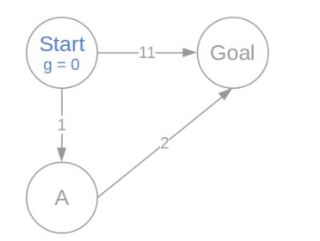
\includegraphics[width=5cm, height=3cm]{figuras/coste1.JPG}
      \caption{Ejemplo de Grafo de Búsqueda de costo uniforme (UCS).}
      \label{fcoste1} 
      \end{center}
\end{figure}

Al principio, solo el nodo de inicio está en la frontera y su \textit{g} valor es 0.

\begin{figure}[H]
 \begin{center}
       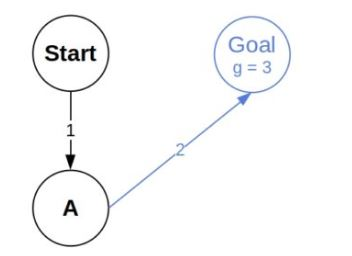
\includegraphics[width=5cm, height=3cm]{figuras/coste2.JPG}
      \caption{Ejemplo de Grafo de Búsqueda de costo uniforme (UCS).}
      \label{fcoste2} 
      \end{center}
\end{figure}

Después de expandir \textit{Goal}, se observa en la Figura ~\ref{fcoste2}  que pasa la prueba del objetivo, por lo que concluimos que la ruta óptima es \textit{Start{-}A{-}Goal}.

A continuación, una investigación respecto a la Búsqueda de costo uniforme:

\begin{enumerate}
\item En el articulo titulado \textit{“Selección de ubicación de instalaciones de construcción para proyectos de mantenimiento de infraestructura lineal urbana utilizando el método de búsqueda de costo uniforme”}, Mansour, A.G., Eid, M.S. \& Elbeltagi, E.E \citep{mansour} presentan un modelo para asignar ubicaciones de instalaciones de construcción (CFL) a cada segmento de trabajo en proyectos de infraestructura lineal que se caracterizan por cambios frecuentes de ubicación del sitio de construcción a medida que avanza el trabajo. El modelo propuesto utiliza un algoritmo de búsqueda de árbol—Búsqueda uniforme de costos (UCS)—que garantiza una solución óptima global. El modelo propuesto, con el algoritmo de poda, es capaz de resolver un problema de espacio de solución de 4 billones en menos de 3000 ms utilizando una máquina de 8 GB de RAM y 2 GHz. El modelo propuesto se puede integrar en los procesos de toma de decisiones de planificación y diseño del sitio para proyectos de infraestructura lineal para reducir el costo general del diseño del sitio.
\end{enumerate}

\subsection{\underline{\textbf{Búsqueda voraz (greedy)}}}
La Universidad Veracruzana en el curso de Inteligencia Artificial \citep{vera} establece que la búsqueda voraz greedy expande el nodo más cercano al objetivo, asumiendo que probablemente conduzca más rápidamente a la solución.
La función de evaluación $f(n)$ es la función heurística $h(n)$
\begin{center}
    \par $f(n) = h(n)$
\end{center}
\par donde $h(n) =$ costo estimado del camino más barato desde el nodo n hasta el objetivo.

El término Voraz (Greedy) ó Avaro es porque en cada paso trata de situarse tan cerca del objetivo como pueda, seleccionando el nodo con menor función de evaluación $f(n)$.

\begin{itemize}
\item No necesariamente brinda la solución óptima.
\item Al igual que los otros métodos es necesario verificar los “callejones sin salidas” (no expandir estados repetidos).
\end{itemize}

A continuación, una investigación respecto a la búsqueda voraz (greedy):
\begin{enumerate}
\item La investigación cuyo título es \textit{“Estimación robusta de canales de comunicaciones de ultra banda ancha"} \citep{yanez2019estimacion}, explica que los sistemas UWB (ultra-wide band) transmiten señales a baja potencia a través de canales de comunicaciones que operan en entornos cerrados y en distancias cortas, lo que origina múltiples trayectorias de propagación.

Además, el ruido que afecta a estos canales se puede caracterizar mediante el uso de modelos estadísticos de colas más pesadas que las exhibidas por la distribución gaussiana. En este trabajo, se propone un enfoque robusto para la estimación de los parámetros de los canales UWB basado en la mediana ponderada.

Específicamente, se desarrolla un \textbf{algoritmo de búsqueda voraz}, ver Figura ~\ref{fgre}, que aprovecha la característica poco densa de la respuesta impulsiva del canal, donde las ganancias y los retardos de los canales relevantes se determinan aplicando la mediana ponderada sobre una versión escalada y desplazada de la señal recibida.

El algoritmo propuesto se evalúa usando extensas simulaciones en las que el rendimiento del algoritmo propuesto supera el desempeño del algoritmo de búsqueda voraz tradicional para diferentes niveles de ruido impulsivo.

\begin{figure}[H]
 \begin{center}
       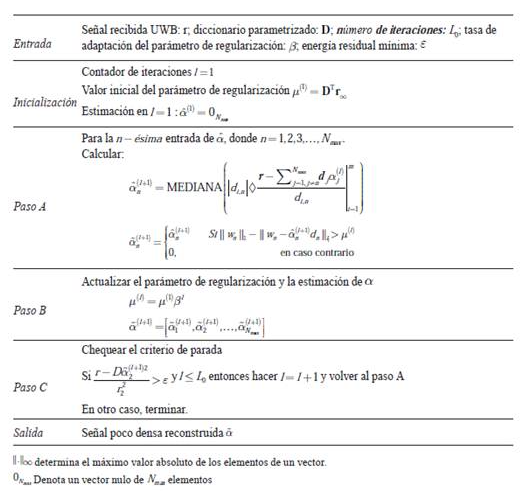
\includegraphics[width=7.5cm, height=6cm]{figuras/voraz.PNG}
      \caption{Algoritmo de búsqueda voraz usando mediana ponderada.}
      \label{fgre} 
      \end{center}
\end{figure}
\end{enumerate}
%---------------------------------------------------------------------------
\subsection{\underline{\textbf{Búsqueda A*}}}
A* es un algoritmo de búsqueda inteligente o informada que busca el camino más corto desde un estado inicial al estado meta a través de un espacio de problema, usando una heurística óptima \citep{Algoritm99}.

Como ignora los pasos más “cortos" en algunos casos rinde una solución subóptima.

Los Fundamentos de la búsqueda A* son:
\begin{itemize}
\item Minimiza el costo estimado total de la solución.
\item Evalúa los nodos combinando
 \begin{center}
$g(n)$ y $h(n)$
 \end{center}
\par $g(n):$ costo de haber alcanzado $n$
\par $h(n):$ costo para llegar desde $n$ hasta el objetivo
\par $f(n) = g(n) + h(n) ->$ costo más barato estimado de la solución a través de $n$.
\item En cada paso se expande el nodo con el valor más bajo de $f(n)$, ó sea, de $g(n)+h(n)$.
\item La búsqueda A* es óptima siempre y cuando la función heurística $h(n)$ sea una heurística admisible, es decir nunca sobreestime el costo de alcanzar el objetivo.
\item Son funciones optimistas.
\end{itemize}

Una investigación sobre la búsqueda A* es:

\begin{enumerate}
\item La \textit{“Implementación del Algoritmo A-Star para la Búsqueda de Rutas Cercanas al Punto de Refugio de Evacuación de Tsunami”} \citep{astri2020implementation}, evaluó el Purus Kelurahan de Padang, ciudad de Indonesia, que tiene un área de $0,86 Km2$ que consta de $8 RW$ y $28 RT$, tiene una población de $8.075$ personas con una densidad de $11.875$ que tiene el potencial de verse afectado por desastres si ocurre un tsunami en la ciudad de Padang.

Las personas en esta ciudad siempre están acosadas por el miedo y se sienten amenazadas si ocurre un terremoto o un tsunami. Por esta razón la investigación menciona que es necesario que haya un proceso educativo para que la comunidad tenga una cultura de concientización sobre desastres en forma de un sistema que sea capaz de informar a la comunidad cuál es la zona segura más cercana a la que pueden llegar y la ruta que tienen que recorrer, obsérvese Figura  ~\ref{faster3}.

\begin{figure}[H]
 \begin{center}
       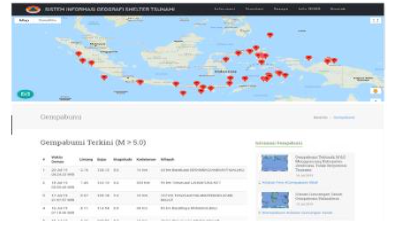
\includegraphics[width=7.5cm, height=4.5cm]{figuras/faster3.PNG}
      \caption{Página del Terremoto.}
      \label{faster3} 
      \end{center}
\end{figure}

Por lo tanto, se creó un sistema de información geográfica (SIG) utilizando el método del Algoritmo A-Star. El \textbf{algoritmo A-Star} utiliza la estimación de distancia más cercana para alcanzar la meta (objetivo) y tiene un valor heurístico que se utiliza como base para la consideración, ver Figura  ~\ref{fpa}. En este sistema hay un camino alternativo y muestra la cantidad de capacidad y la distancia desde el refugio a abordar. 

Los investigadores utilizaron un método descriptivo mediante la recopilación de datos e información sobre rutas de evacuación de tsunamis y refugios en el área de Purus de la ciudad de Padang que ayuda a minimizar las víctimas en casos de desastre.

\begin{figure}[H]
 \begin{center}
       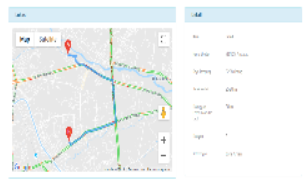
\includegraphics[width=7.5cm, height=4.5cm]{figuras/fpa.PNG}
      \caption{Página de la ruta del refugio más cercano.}
      \label{fpa} 
      \end{center}
\end{figure}
\end{enumerate}
%---------------------------------------------------------------------------
\section{\textbf{Conclusión}}
Este informe presentó información relevante acerca de las cinco estrategias de búsqueda no informadas y son: Búsqueda en amplitud(BFS), Búsqueda en profundidad(DFS), Búsqueda de costo uniforme(UCS) e informadas: Búsqueda voraz (greedy) y Búsqueda A*, se ha explicado los conceptos teóricos relacionados con ellas. Además de permitir conocer algunas investigaciones que se vienen realizando año a año, entendiendo las diversas aplicaciones de ellas en la vida diaria. Concluimos respecto a ello que la mayoría analiza la problemática, establece el proceso y propone resolver problemas utilizando el método correcto en los que para llevarlos a cabo de forma efectiva y eficientemente, utilizan bases teóricas sobre el conocimiento heurístico.
%-------------------------------------------------------
\medskip
\bibliography{refer}
\end{document}